\label{pseudoI}%
\sanglada{%
\rubrik{Pseudovetenskap och ingenjörskonst}
\begin{sangtext}
\sangare{Nef}%
    Lyssna och lyd, din attityd
	är inte sober.
	Prästen med fru lurar dig ju,
	de är teknofober.
	Astrologi, telepati
	är för de veka.
	Var lite sund, skaffa en grund,
	lär dig meka!\radskip

\sangare{Anc}%
    Jag vill bli befriad från materien,
	sväva bland andar och själar.
	Jag vill bli befriad och jag ber igen.
	Släpp tekniksamhällets trälar!
	Jag vill bli befriad från materien,
	uppleva drömfantasier!
	Jag vill bli befriad och jag ser, min vän.
	grå är alla teorier!\radskip
	
	Åh, du gamla dumma moder,
	skippa logiska metoder!
	Dina gudar gråter floder.
	Lösgör ditt roder!\radskip
	
\sangare{Nef}%
    Du har lärt dig fel och om det sker igen,
	får du läsa extra under ferien!\radskip
	
\sangare{Anc}%
    Jag vill bli befriad från materien!\radskip
	
\hfill\emph{Text: Tore K}
\end{sangtext}
\begin{sangtextsingel}
\emph{Pappa jag vill ha en italienare}\hfill\textsc{Musik: Galenskaparna, Arr: Karin S-A}
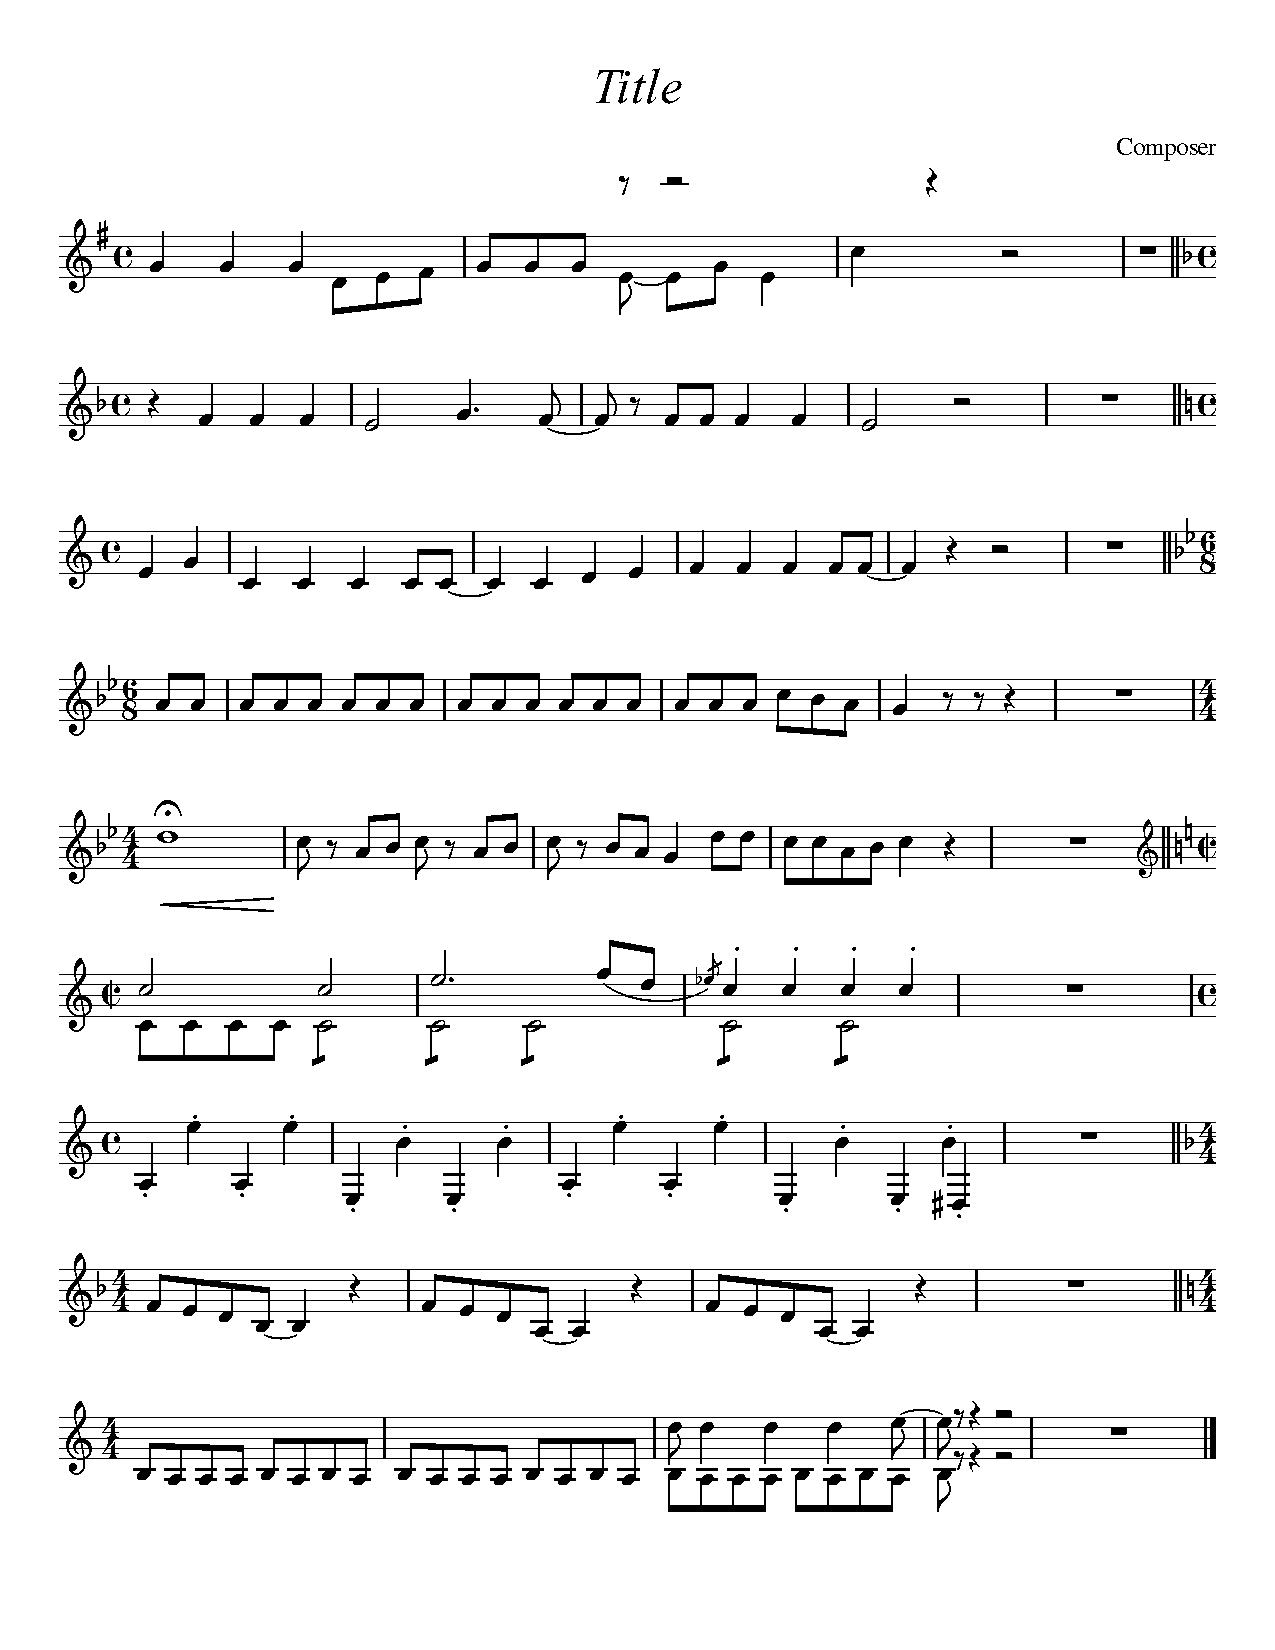
\includegraphics[height=1.60cm, clip,%
trim=1.05cm 22.5cm 5.9cm 3.5cm]{songs/noter_ovr1.pdf}
\end{sangtextsingel}}